% Created 2024-10-13 Sun 23:55
% Intended LaTeX compiler: pdflatex
\documentclass[11pt]{article}
\usepackage[utf8]{inputenc}
\usepackage[T1]{fontenc}
\usepackage{graphicx}
\usepackage{longtable}
\usepackage{wrapfig}
\usepackage{rotating}
\usepackage[normalem]{ulem}
\usepackage{amsmath}
\usepackage{amssymb}
\usepackage{capt-of}
\usepackage{hyperref}
\usepackage[polish]{babel}
\usepackage[T1]{fontenc}
\usepackage[utf8]{inputenc}
\selectlanguage{polish}
\usepackage{caption}
\usepackage{booktabs}
\captionsetup{labelfont=bf}
\usepackage{float}
\author{Piotr Karamon}
\date{14.10.2024r.}
\title{Laboratorium 1 - Współbieżność w Javie}
\hypersetup{
 pdfauthor={Piotr Karamon},
 pdftitle={Laboratorium 1 - Współbieżność w Javie},
 pdfkeywords={},
 pdfsubject={},
 pdfcreator={Emacs 29.2 (Org mode 9.8)}, 
 pdflang={Polish}}

% Setup for code blocks [1/2]

\usepackage{fvextra}

\fvset{%
  commandchars=\\\{\},
  highlightcolor=white!95!black!80!blue,
  breaklines=true,
  breaksymbol=\color{white!60!black}\tiny\ensuremath{\hookrightarrow}}

% Make line numbers smaller and grey.
\renewcommand\theFancyVerbLine{\footnotesize\color{black!40!white}\arabic{FancyVerbLine}}

\usepackage{xcolor}

% In case engrave-faces-latex-gen-preamble has not been run.
\providecolor{EfD}{HTML}{f7f7f7}
\providecolor{EFD}{HTML}{28292e}

% Define a Code environment to prettily wrap the fontified code.
\usepackage[breakable,xparse]{tcolorbox}
\DeclareTColorBox[]{Code}{o}%
{colback=EfD!98!EFD, colframe=EfD!95!EFD,
  fontupper=\footnotesize\setlength{\fboxsep}{0pt},
  colupper=EFD,
  IfNoValueTF={#1}%
  {boxsep=2pt, arc=2.5pt, outer arc=2.5pt,
    boxrule=0.5pt, left=2pt}%
  {boxsep=2.5pt, arc=0pt, outer arc=0pt,
    boxrule=0pt, leftrule=1.5pt, left=0.5pt},
  right=2pt, top=1pt, bottom=0.5pt,
  breakable}

% Support listings with captions
\usepackage{float}
\floatstyle{plain}
\newfloat{listing}{htbp}{lst}
\newcommand{\listingsname}{Listing}
\floatname{listing}{\listingsname}
\newcommand{\listoflistingsname}{List of Listings}
\providecommand{\listoflistings}{\listof{listing}{\listoflistingsname}}


% Setup for code blocks [2/2]: syntax highlighting colors

\newcommand\efstrut{\vrule height 2.1ex depth 0.8ex width 0pt}
\definecolor{EFD}{HTML}{383a42}
\definecolor{EfD}{HTML}{fafafa}
\newcommand{\EFD}[1]{\textcolor{EFD}{#1}} % default
\newcommand{\EFvp}[1]{#1} % variable-pitch
\definecolor{EFh}{HTML}{383a42}
\newcommand{\EFh}[1]{\textcolor{EFh}{#1}} % shadow
\definecolor{EFsc}{HTML}{556b2f}
\newcommand{\EFsc}[1]{\textcolor{EFsc}{#1}} % success
\definecolor{EFw}{HTML}{986801}
\newcommand{\EFw}[1]{\textcolor{EFw}{#1}} % warning
\definecolor{EFe}{HTML}{e45649}
\newcommand{\EFe}[1]{\textcolor{EFe}{#1}} % error
\definecolor{EFl}{HTML}{014980}
\newcommand{\EFl}[1]{\textcolor{EFl}{\textbf{#1}}} % link
\definecolor{EFlv}{HTML}{8b008b}
\newcommand{\EFlv}[1]{\textcolor{EFlv}{\textbf{#1}}} % link-visited
\definecolor{EFhi}{HTML}{f0f0f0}
\definecolor{Efhi}{HTML}{014980}
\newcommand{\EFhi}[1]{\colorbox{Efhi}{\efstrut{}\textcolor{EFhi}{#1}}} % highlight
\definecolor{EFc}{HTML}{556b2f}
\newcommand{\EFc}[1]{\textcolor{EFc}{#1}} % font-lock-comment-face
\definecolor{EFcd}{HTML}{556b2f}
\newcommand{\EFcd}[1]{\textcolor{EFcd}{#1}} % font-lock-comment-delimiter-face
\definecolor{EFs}{HTML}{8a3b3c}
\newcommand{\EFs}[1]{\textcolor{EFs}{#1}} % font-lock-string-face
\definecolor{EFd}{HTML}{485a27}
\newcommand{\EFd}[1]{\textcolor{EFd}{\textit{#1}}} % font-lock-doc-face
\newcommand{\EFm}[1]{#1} % font-lock-doc-markup-face
\newcommand{\EFk}[1]{\textbf{#1}} % font-lock-keyword-face
\newcommand{\EFb}[1]{\textbf{#1}} % font-lock-builtin-face
\newcommand{\EFf}[1]{\textbf{#1}} % font-lock-function-name-face
\newcommand{\EFv}[1]{#1} % font-lock-variable-name-face
\newcommand{\EFt}[1]{\textbf{#1}} % font-lock-type-face
\newcommand{\EFo}[1]{#1} % font-lock-constant-face
\definecolor{EFwr}{HTML}{986801}
\newcommand{\EFwr}[1]{\textcolor{EFwr}{#1}} % font-lock-warning-face
\newcommand{\EFnc}[1]{\textbf{#1}} % font-lock-negation-char-face
\newcommand{\EFpp}[1]{\textbf{#1}} % font-lock-preprocessor-face
\newcommand{\EFrc}[1]{\textbf{#1}} % font-lock-regexp-grouping-construct
\newcommand{\EFrb}[1]{\textbf{#1}} % font-lock-regexp-grouping-backslash
\definecolor{Efob}{HTML}{e7e7e7}
\newcommand{\EFob}[1]{\colorbox{Efob}{\efstrut{}#1}} % org-block
\definecolor{Efobb}{HTML}{e7e7e7}
\newcommand{\EFobb}[1]{\colorbox{Efobb}{\efstrut{}\textit{#1}}} % org-block-begin-line
\definecolor{Efobe}{HTML}{e7e7e7}
\newcommand{\EFobe}[1]{\colorbox{Efobe}{\efstrut{}\textit{#1}}} % org-block-end-line
\newcommand{\EFOa}[1]{\textbf{#1}} % outline-1
\newcommand{\EFOb}[1]{\textbf{#1}} % outline-2
\newcommand{\EFOc}[1]{\textbf{#1}} % outline-3
\newcommand{\EFOd}[1]{\textbf{#1}} % outline-4
\newcommand{\EFOe}[1]{\textbf{#1}} % outline-5
\newcommand{\EFOf}[1]{\textbf{#1}} % outline-6
\newcommand{\EFOg}[1]{\textbf{#1}} % outline-7
\newcommand{\EFOh}[1]{\textbf{#1}} % outline-8
\definecolor{EFhn}{HTML}{8a3b3c}
\newcommand{\EFhn}[1]{\textcolor{EFhn}{\textbf{#1}}} % highlight-numbers-number
\newcommand{\EFhq}[1]{#1} % highlight-quoted-quote
\newcommand{\EFhs}[1]{#1} % highlight-quoted-symbol
\definecolor{EFrda}{HTML}{014980}
\newcommand{\EFrda}[1]{\textcolor{EFrda}{#1}} % rainbow-delimiters-depth-1-face
\definecolor{EFrdb}{HTML}{a626a4}
\newcommand{\EFrdb}[1]{\textcolor{EFrdb}{#1}} % rainbow-delimiters-depth-2-face
\definecolor{EFrdc}{HTML}{556b2f}
\newcommand{\EFrdc}[1]{\textcolor{EFrdc}{#1}} % rainbow-delimiters-depth-3-face
\definecolor{EFrdd}{HTML}{b751b6}
\newcommand{\EFrdd}[1]{\textcolor{EFrdd}{#1}} % rainbow-delimiters-depth-4-face
\definecolor{EFrde}{HTML}{4db5bd}
\newcommand{\EFrde}[1]{\textcolor{EFrde}{#1}} % rainbow-delimiters-depth-5-face
\definecolor{EFrdf}{HTML}{014980}
\newcommand{\EFrdf}[1]{\textcolor{EFrdf}{#1}} % rainbow-delimiters-depth-6-face
\definecolor{EFrdg}{HTML}{a626a4}
\newcommand{\EFrdg}[1]{\textcolor{EFrdg}{#1}} % rainbow-delimiters-depth-7-face
\definecolor{EFrdh}{HTML}{556b2f}
\newcommand{\EFrdh}[1]{\textcolor{EFrdh}{#1}} % rainbow-delimiters-depth-8-face
\definecolor{EFrdi}{HTML}{b751b6}
\newcommand{\EFrdi}[1]{\textcolor{EFrdi}{#1}} % rainbow-delimiters-depth-9-face
\definecolor{EFany}{HTML}{986801}
\definecolor{Efany}{HTML}{986801}
\newcommand{\EFany}[1]{\colorbox{Efany}{\efstrut{}\textcolor{EFany}{#1}}} % ansi-color-yellow
\definecolor{EFanr}{HTML}{e45649}
\definecolor{Efanr}{HTML}{e45649}
\newcommand{\EFanr}[1]{\colorbox{Efanr}{\efstrut{}\textcolor{EFanr}{#1}}} % ansi-color-red
\definecolor{EFanb}{HTML}{fafafa}
\newcommand{\EFanb}[1]{\textcolor{EFanb}{#1}} % ansi-color-black
\definecolor{EFang}{HTML}{556b2f}
\definecolor{Efang}{HTML}{556b2f}
\newcommand{\EFang}[1]{\colorbox{Efang}{\efstrut{}\textcolor{EFang}{#1}}} % ansi-color-green
\definecolor{EFanB}{HTML}{014980}
\definecolor{EfanB}{HTML}{014980}
\newcommand{\EFanB}[1]{\colorbox{EfanB}{\efstrut{}\textcolor{EFanB}{#1}}} % ansi-color-blue
\definecolor{EFanc}{HTML}{0184bc}
\definecolor{Efanc}{HTML}{0184bc}
\newcommand{\EFanc}[1]{\colorbox{Efanc}{\efstrut{}\textcolor{EFanc}{#1}}} % ansi-color-cyan
\definecolor{Efanw}{HTML}{383a42}
\newcommand{\EFanw}[1]{\colorbox{Efanw}{\efstrut{}#1}} % ansi-color-white
\definecolor{EFanm}{HTML}{a626a4}
\definecolor{Efanm}{HTML}{a626a4}
\newcommand{\EFanm}[1]{\colorbox{Efanm}{\efstrut{}\textcolor{EFanm}{#1}}} % ansi-color-magenta
\definecolor{EFANy}{HTML}{a77e27}
\definecolor{EfANy}{HTML}{a77e27}
\newcommand{\EFANy}[1]{\colorbox{EfANy}{\efstrut{}\textcolor{EFANy}{#1}}} % ansi-color-bright-yellow
\definecolor{EFANr}{HTML}{e86f64}
\definecolor{EfANr}{HTML}{e86f64}
\newcommand{\EFANr}[1]{\colorbox{EfANr}{\efstrut{}\textcolor{EFANr}{#1}}} % ansi-color-bright-red
\definecolor{EFANb}{HTML}{f0f0f0}
\definecolor{EfANb}{HTML}{dfdfdf}
\newcommand{\EFANb}[1]{\colorbox{EfANb}{\efstrut{}\textcolor{EFANb}{#1}}} % ansi-color-bright-black
\definecolor{EFANg}{HTML}{6e814e}
\definecolor{EfANg}{HTML}{6e814e}
\newcommand{\EFANg}[1]{\colorbox{EfANg}{\efstrut{}\textcolor{EFANg}{#1}}} % ansi-color-bright-green
\definecolor{EFANB}{HTML}{276493}
\definecolor{EfANB}{HTML}{276493}
\newcommand{\EFANB}[1]{\colorbox{EfANB}{\efstrut{}\textcolor{EFANB}{#1}}} % ansi-color-bright-blue
\definecolor{EFANc}{HTML}{2796c6}
\definecolor{EfANc}{HTML}{2796c6}
\newcommand{\EFANc}[1]{\colorbox{EfANc}{\efstrut{}\textcolor{EFANc}{#1}}} % ansi-color-bright-cyan
\definecolor{EFANw}{HTML}{1b2229}
\definecolor{EfANw}{HTML}{1b2229}
\newcommand{\EFANw}[1]{\colorbox{EfANw}{\efstrut{}\textcolor{EFANw}{#1}}} % ansi-color-bright-white
\definecolor{EFANm}{HTML}{b346b1}
\definecolor{EfANm}{HTML}{b346b1}
\newcommand{\EFANm}[1]{\colorbox{EfANm}{\efstrut{}\textcolor{EFANm}{#1}}} % ansi-color-bright-magenta
\begin{document}

\maketitle
\section*{Treści zadań}
\label{sec:orgf8834f6}
\subsection*{Zadanie 1}
\label{sec:org3f5ea0c}
Napisać program (szkielet), który uruchamia 2 wątki, z których jeden zwiększa
wartość zmiennej całkowitej o 1, drugi wątek zmniejsza wartość o 1. Zakładając
że na początku wartość zmiennej Counter była 0, chcielibyśmy wiedzieć jaka
będzie wartość tej zmiennej po wykonaniu 10000 operacji zwiększania i
zmniejszania przez obydwa wątki.
\subsection*{Zadanie 2}
\label{sec:orgb40bca8}
Na podstawie 100 wykonań programu z p.1, stworzyć histogram końcowych wartości zmiennej Counter.
\subsection*{Zadanie 3}
\label{sec:org851689d}
Spróbować wprowadzić mechanizm do programu z p.1, który zagwarantowałby przewidywalną końcową wartość zmiennej Counter. Nie używać żadnych systemowych mechanizmów, tylko swój autorski.
\subsection*{Zadanie dodatkowe}
\label{sec:org8871b03}
W systemie działa N wątków, które dzielą obiekt licznika (początkowy stan licznika = 0).

Każdy wątek wykonuje w pętli 5 razy inkrementację licznika. Zakładamy, że inkrementacja składa się z sekwencji trzech instrukcji: \texttt{read}, \texttt{inc}, \texttt{write} (odczyt z pamięci, zwiększenie o 1, zapis do pamięci). Wątki nie są synchronizowane.

\begin{enumerate}
\item Jaka jest teoretycznie najmniejsza wartość licznika po zakończeniu działania wszystkich wątków i jaka kolejność instrukcji (przeplot) do niej prowadzi?
\item Spróbować znaleźć dowód, że będzie to zawsze najmniejsza wartość.
\end{enumerate}
\section*{Zadanie 1}
\label{sec:orgf387df0}
W celu wykonania eksperymentu tworzymy dwie klasy, które dziedziczą po klasie
\texttt{Thread}. Nadpisujemy w nich metodę \texttt{run} gdzie umieszczamy logikę jaką chcemy by nasze
wątki wykonywały. Wątki uruchamiamy metodą \texttt{start()}. By sprawdzić końcową wartość
zmiennej \texttt{Counter} musimy zaczekać aż wątki skończą pracę, używamy do tego
metody \texttt{join()}.


\begin{Code}
\begin{Verbatim}
\color{EFD}\EFcd{//} \EFc{Race.java}
\EFcd{//} \EFc{Wyscig}

\EFk{class} \EFt{Counter} \EFrda{\{}
    \EFk{private} \EFt{int} \EFv{\_val};

    \EFk{public} Counter\EFrdb{(}\EFt{int} \EFv{n}\EFrdb{)} \EFrdb{\{}
        \_val = n;
    \EFrdb{\}}

    \EFk{public} \EFt{void} \EFf{inc}\EFrdb{(}\EFrdb{)} \EFrdb{\{}
        \_val++;
    \EFrdb{\}}

    \EFk{public} \EFt{void} \EFf{dec}\EFrdb{(}\EFrdb{)} \EFrdb{\{}
        \_val--;
    \EFrdb{\}}

    \EFk{public} \EFt{int} \EFf{value}\EFrdb{(}\EFrdb{)} \EFrdb{\{}
        \EFk{return} \_val;
    \EFrdb{\}}
\EFrda{\}}

\EFcd{//} \EFc{Watek, ktory inkrementuje licznik 100.000 razy}
\EFk{class} \EFt{IThread} \EFk{extends} \EFt{Thread} \EFrda{\{}
    \EFk{private} \EFk{final} \EFt{Counter} \EFv{counter};

    \EFk{public} IThread\EFrdb{(}Counter counter\EFrdb{)} \EFrdb{\{}
        \EFk{this}.counter = counter;
    \EFrdb{\}}

    @Override
    \EFk{public} \EFt{void} \EFf{run}\EFrdb{(}\EFrdb{)} \EFrdb{\{}
        \EFk{for} \EFrdc{(}\EFt{int} \EFv{i} = \EFhn{0}; i < 100\_000; i++\EFrdc{)} \EFrdc{\{}
            counter.inc\EFrdd{(}\EFrdd{)};
        \EFrdc{\}}
    \EFrdb{\}}
\EFrda{\}}

\EFcd{//} \EFc{Watek, ktory dekrementuje licznik 100.000 razy}
\EFk{class} \EFt{DThread} \EFk{extends} \EFt{Thread} \EFrda{\{}
    \EFk{private} \EFk{final} \EFt{Counter} \EFv{counter};

    \EFk{public} DThread\EFrdb{(}Counter counter\EFrdb{)} \EFrdb{\{}
        \EFk{this}.counter = counter;
    \EFrdb{\}}

    @Override
    \EFk{public} \EFt{void} \EFf{run}\EFrdb{(}\EFrdb{)} \EFrdb{\{}
        \EFk{for} \EFrdc{(}\EFt{int} \EFv{i} = \EFhn{0}; i < 100\_000; i++\EFrdc{)} \EFrdc{\{}
            counter.dec\EFrdd{(}\EFrdd{)};
        \EFrdc{\}}
    \EFrdb{\}}
\EFrda{\}}

\EFk{public} \EFk{class} \EFt{Race} \EFrda{\{}

    \EFk{public} \EFk{static} \EFt{void} \EFf{main}\EFrdb{(}\EFt{String}\EFrdc{[}\EFrdc{]} \EFv{args}\EFrdb{)} \EFrdb{\{}
        \EFt{Counter} \EFv{cnt} = \EFk{new} \EFt{Counter}\EFrdc{(}\EFhn{0}\EFrdc{)};

        \EFt{IThread} \EFv{incThread} = \EFk{new} \EFt{IThread}\EFrdc{(}cnt\EFrdc{)};
        \EFt{DThread} \EFv{decThread} = \EFk{new} \EFt{DThread}\EFrdc{(}cnt\EFrdc{)};

        incThread.start\EFrdc{(}\EFrdc{)};
        decThread.start\EFrdc{(}\EFrdc{)};

        \EFk{try} \EFrdc{\{}
            incThread.join\EFrdd{(}\EFrdd{)};
            decThread.join\EFrdd{(}\EFrdd{)};
        \EFrdc{\}} \EFk{catch} \EFrdc{(}InterruptedException e\EFrdc{)} \EFrdc{\{}
            e.printStackTrace\EFrdd{(}\EFrdd{)};
        \EFrdc{\}}

        System.out.println\EFrdc{(}\EFs{"stan="} + cnt.value\EFrdd{(}\EFrdd{)}\EFrdc{)};
    \EFrdb{\}}
\EFrda{\}}

\end{Verbatim}
\end{Code}

W wyniku uruchomienia otrzymujemy następujące wyjście:
\begin{tcolorbox}
\begin{Verbatim}
stan=1955
\end{Verbatim}


\end{tcolorbox}\textbf{Wnioski}: Jest to wynik znacznie odbiegający od spodziewanego zera.  Mamy tutaj do
czynienia z wyścigiem, czyli sytuacją przy której więcej niż jeden wątek
korzysta jednocześnie z zasobu współdzielonego, przy czym co najmniej jeden
próbuje go zmienić. Wyścig sprawia, że nasz program staje się
niedeterministyczny. Wątki wykonują operacje zwiększania i zmniejszania na
zmiennej \texttt{Counter} bez synchronizacji. Może to prowadzić do sytuacji, w której
jeden wątek odczytuje wartość Counter, podczas gdy drugi wątek ją zmienia, co
prowadzi do utraty niektórych operacji.
\section*{Zadanie 2}
\label{sec:org9a7dde0}
Program z zadania 1 uruchamiamy 100 razy w celu stworzenia histogramu.
Korzystamy z powłoki \texttt{bash} oraz prostej komendy w celu zebrania danych.

\begin{Code}
\begin{Verbatim}
\color{EFD}\EFk{for} i \EFk{in} \EFrda{\{}1..100\EFrda{\}}; \EFk{do} ./gradlew run |  \EFt{grep} -E -o \EFs{'stan=.*'} | sed \EFs{'s/stan=//'} >> output.txt; \EFk{done}
\end{Verbatim}
\end{Code}

Z otrzymanych danych w pliku \texttt{output.txt} tworzymy histogram.

\begin{figure}[H]
\centering
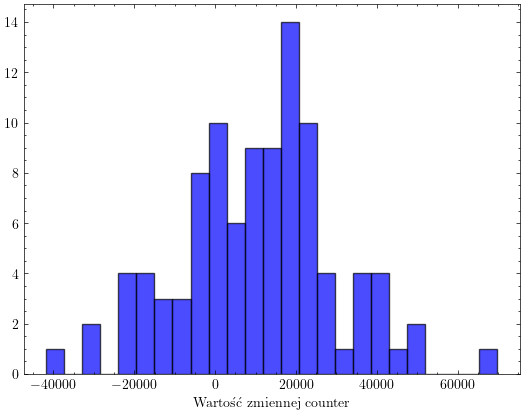
\includegraphics[width=.9\linewidth]{histogram.png}
\caption{\label{}Histogram powstały ze 100 uruchomień programu z zadania 1.}
\end{figure}

\textbf{Wnioski}: Widzimy bardzo duży rozrzut wartości. Co ciekawe rozkład zdaje się być niesymetryczny względem zera.
Histogram pokazuje fakt, iż obecnie bez żadnej synchronizacji nasz program działa w bardzo losowy i
nieprzewidywalny sposób. Jednakże zgodnie z naszą intuicją najwięcej wyników znajduje się blisko zera.
\section*{Zadanie 3}
\label{sec:orgc4a985a}
Celem zadania jest wprowadzenie autorskiego mechanizmu do programu z zadania 1, który
zagwarantuje nam deterministyczny wynik.

To co możemy zrobić to wymuszenie kolejności typu: inc, dec, inc, dec, itd.
Do tego celu potrzebujemy wspólnej zmiennej:

\begin{Code}
\begin{Verbatim}
\color{EFD}\EFk{public} \EFk{static} \EFk{volatile} \EFt{int} \EFv{turn} = \EFhn{0};
\end{Verbatim}
\end{Code}

Wartość 0 oznacza, że wątek inkrementujący ma wykonać jedno \texttt{inc()}.
Wartość 1 oznacza, że wątek dekrementujący ma wykonać jedno \texttt{dec()}.
Korzystamy tutaj ze słowa kluczowego \texttt{volatile}. Dzięki niemu zmiany tej zmiennej są
natychmiast widoczne dla innych wątków. To słowo zapobiega również optymalizacji
polegającej na pobraniu tej zmiennej z pamięci cache.

Potrzebna jest zmiana metod \texttt{run()} w naszych wątkach. Będziemy po prostu czekać w
pętli, aż nie najdzie na nas kolej.

\begin{Code}
\begin{Verbatim}
\color{EFD}\EFk{class} \EFt{IThread} \EFk{extends} \EFt{Thread} \EFrda{\{}
    \EFk{private} \EFk{final} \EFt{Counter} \EFv{counter};

    \EFk{public} IThread\EFrdb{(}Counter counter\EFrdb{)} \EFrdb{\{}
        \EFk{this}.counter = counter;
    \EFrdb{\}}

    @Override
    \EFk{public} \EFt{void} \EFf{run}\EFrdb{(}\EFrdb{)} \EFrdb{\{}
        \EFk{for} \EFrdc{(}\EFt{int} \EFv{i} = \EFhn{0}; i < 100\_000; i++\EFrdc{)} \EFrdc{\{}
            \EFk{while}\EFrdd{(}\EFo{true}\EFrdd{)} \EFrdd{\{}
                \EFk{if} \EFrda{(}Race.turn == \EFhn{0}\EFrda{)} \EFrda{\{}
                    counter.inc\EFrdb{(}\EFrdb{)};
                    Race.turn = \EFhn{1};
                    \EFk{break};
                \EFrda{\}}
            \EFrdd{\}}

        \EFrdc{\}}
    \EFrdb{\}}
\EFrda{\}}

\EFk{class} \EFt{DThread} \EFk{extends} \EFt{Thread} \EFrda{\{}
    \EFk{private} \EFk{final} \EFt{Counter} \EFv{counter};

    \EFk{public} DThread\EFrdb{(}Counter counter\EFrdb{)} \EFrdb{\{}
        \EFk{this}.counter = counter;
    \EFrdb{\}}

    @Override
    \EFk{public} \EFt{void} \EFf{run}\EFrdb{(}\EFrdb{)} \EFrdb{\{}
        \EFk{for} \EFrdc{(}\EFt{int} \EFv{i} = \EFhn{0}; i < 100\_000; i++\EFrdc{)} \EFrdc{\{}
            \EFk{while}\EFrdd{(}\EFo{true}\EFrdd{)} \EFrdd{\{}
                \EFk{if} \EFrda{(}Race.turn == \EFhn{1}\EFrda{)} \EFrda{\{}
                    counter.dec\EFrdb{(}\EFrdb{)};
                    Race.turn = \EFhn{0};
                    \EFk{break};
                \EFrda{\}}
            \EFrdd{\}}
        \EFrdc{\}}
    \EFrdb{\}}
\EFrda{\}}
\end{Verbatim}
\end{Code}

Testujemy nasze rozwiązanie uruchamiając je 200 razy.
\begin{Code}
\begin{Verbatim}
\color{EFD}\EFk{public} \EFk{static} \EFt{void} \EFf{main}\EFrda{(}\EFt{String}\EFrdb{[}\EFrdb{]} \EFv{args}\EFrda{)} \EFrda{\{}
    \EFt{var} \EFv{allZeros} = IntStream.range\EFrdb{(}\EFhn{0}, \EFhn{200}\EFrdb{)}.map\EFrdb{(}i -> runSample\EFrdc{(}\EFrdc{)}\EFrdb{)}.allMatch\EFrdb{(}i -> i == \EFhn{0}\EFrdb{)};
    System.out.println\EFrdb{(}\EFs{"all zeros = "}+allZeros\EFrdb{)};
\EFrda{\}}

\EFk{private} \EFk{static} \EFt{int} \EFf{runSample}\EFrda{(}\EFrda{)} \EFrda{\{}
    \EFt{Counter} \EFv{cnt} = \EFk{new} \EFt{Counter}\EFrdb{(}\EFhn{0}\EFrdb{)};

    Race.turn = \EFhn{0};

    \EFt{IThread} \EFv{incThread} = \EFk{new} \EFt{IThread}\EFrdb{(}cnt\EFrdb{)};
    \EFt{DThread} \EFv{decThread} = \EFk{new} \EFt{DThread}\EFrdb{(}cnt\EFrdb{)};

    incThread.start\EFrdb{(}\EFrdb{)};
    decThread.start\EFrdb{(}\EFrdb{)};

    \EFk{try} \EFrdb{\{}
            incThread.join\EFrdc{(}\EFrdc{)};
            decThread.join\EFrdc{(}\EFrdc{)};
    \EFrdb{\}} \EFk{catch} \EFrdb{(}InterruptedException e\EFrdb{)} \EFrdb{\{}
            e.printStackTrace\EFrdc{(}\EFrdc{)};
    \EFrdb{\}}

    \EFk{return} cnt.value\EFrdb{(}\EFrdb{)};
\EFrda{\}}
\end{Verbatim}
\end{Code}

Otrzymane wyjście:
\begin{tcolorbox}
\begin{Verbatim}
all zeros = true
\end{Verbatim}


\end{tcolorbox}\textbf{Wnioski}: Nasze rozwiązanie zdaje się działać, jednakże jest ono wysoce nieefektywne głównie dlatego, że
wątki używają pętli \texttt{while (true)} do oczekiwania na zmianę stanu zmiennej \texttt{turn}.
To prowadzi do "busy waiting", gdzie wątki nie wykonują żadnej użytecznej
pracy, a jedynie ciągle sprawdzają stan zmiennej. To jest bardzo nieefektywne z
perspektywy zasobów procesora. Dlatego realistycznie powinniśmy skorzystać z gotowych
mechanizmów takich jak:
\begin{itemize}
\item bloki/funkcje \texttt{synchronized}
\item \texttt{ReentranLock}
\item \texttt{Semaphore}
\item zmienne atomowe w tym przypadku \texttt{AtomicInteger}
\end{itemize}
\section*{Zadanie dodatkowe}
\label{sec:org543969a}
Idea rozwiązania polega na wczesnym wykonaniu instrukcji \texttt{read} oraz \texttt{inc} przez jeden wątek,
następnie na pozwoleniu na pracę innych wątków, których praca zostanie nadpisana
po wywołaniu \texttt{write} przez ten wczesny wątek.


Dla \(N=1\) problem staje się całkowicie sekwencyjny, zatem otrzymamy wartość równą 5.
Dla \(N > 1\) najmniejsza możliwa wartość licznika to 2.
Odpowiadający przeplot:

\begin{center}
\begin{tabular}{ll}
wątek & instrukcja\\
\hline
\(w_1\) & read\\
\(w_1\) & inc\\
\(w_3\)..\(w_N\) & wykonują pełne 5 iteracji\\
\(w_2\) & wykonuje pełne 4 iteracji\\
\(w_1\) & write(teraz \texttt{counter=1})\\
\(w_2\) & read(wczytanie \texttt{counter=1})\\
\(w_1\) & wykonuje pozostałe 4 iteracje w całości\\
\(w_2\) & inc\\
\(w_2\) & write(wpisanie \texttt{counter=2})\\
\end{tabular}
\end{center}


Najmniejsza możliwa wartość licznika nie może być równa 0,
ponieważ niezależnie od przeplotu końcową instrukcją jest \texttt{write},
odpowiadający mu \texttt{read} (ten sam wątek, ta sama iteracja) wczytał liczbę
która jest \(\ge 0\), przez to dzięki \texttt{inc} wpiszemy wartość \(>=1\).

Teraz zastanówmy się, czy możliwe jest by licznik miał na końcu wartość 1.
Zrobimy dowód nie wprost.

Jeżeli na końcu dostaliśmy wartość 1, to ostatnia instrukcja \texttt{write}, wpisała
wartość 1(niech wykona ją wątek \(w_{a}\)).  Odpowiadający tej instrukcji \texttt{read}
(ten sam wątek, ta sama iteracja) musiał wczytać 0. To oznacza, że żaden wątek
nie mógł wcześniej niż ta instrukcja \texttt{read} wykonać instrukcji \texttt{write} (bo wczytana
wartość byłaby \(> 0\)). Ale to oznacza, że również wątek \(w_a\) nie mógł wykonać
instrukcji \texttt{write}, co jest sprzecznością, ponieważ w momencie wykonania ostatniej
swojej instrukcji \texttt{read} jest w 5 iteracji, a co za tym idzie wykonał on 4 instrukcje \texttt{write}.

\textbf{Wnioski}: Możliwe przeploty potrafią prowadzić do bardzo zaskakujących wyników.
Opisany powyżej przeplot jest kompletnie nieintuicyjny oraz bardzo mało prawdopodobny,
fakt jego istnienia pokazuje trudność programowania współbieżnego oraz analizy
algorytmów współbieżnych.
\section*{Bibliografia}
\label{sec:org2741e60}
\begin{itemize}
\item Bill Venners: \emph{Inside the Java Virtual Machine Chapter 20}
\item \href{https://docs.oracle.com/javase/tutorial/essential/concurrency/atomic.html}{Atomic Access}
\item \href{https://download.java.net/java/early\_access/valhalla/docs/api/java.base/java/lang/Thread.html}{Dokumentacja klasy thread}
\end{itemize}
\end{document}
